\section{Mechanisms}
\label{sec:mechanisms}

The results establish that lucky loser entry causes gains in tournament access, ranking point accumulation, and no change in Elo ratings. This section synthesizes these findings through three channels: access, access cascade, and match-level performance conditional on opponent strength.

\subsection{Access Channel}
\label{sec:mechanisms_access}

The most direct mechanism is that LL entry provides a main draw appearance that the player would not otherwise have received. This appearance generates ranking points proportional to the round reached, which in turn improve the player's position in the rolling 52-week ranking. The improved ranking may cross direct-entry thresholds for subsequent tournaments---particularly at lower-tier events (ATP/WTA 250) where the entry threshold is more accessible. The evidence supports this channel: on the ATP tour, treated players enter 1.1 more main draws over 26 weeks ($p = 0.006$) and play 1.8 more matches at 250+ events ($p = 0.010$).

The Elo null establishes that the access channel operates through the ranking system, not through improved playing skill. Elo ratings adjust for opponent quality: a player who enters more tournaments but faces proportionally tougher opponents will not see their Elo rise unless their actual match performance improves. The null Elo result at all horizons, on both tours, confirms that the additional tournament access does not translate into better quality-adjusted match outcomes.

\subsection{Access Cascade}
\label{sec:mechanisms_cascade}

The dose-response results trace how the access channel compounds through the ranking system. A player who receives the LL slot but loses in the first round earns minimal ranking points (10 at a Grand Slam). This is not enough to meaningfully change their position or gain access to subsequent main draws. Their outcomes are indistinguishable from controls.

A player who wins one or more main draw matches earns substantially more points (45 for a second-round loss, 90 for a third-round loss at a Grand Slam). This shifts their position enough to cross direct-entry thresholds at lower-tier events, generating additional main draw entries over the next 26 weeks. Each subsequent entry provides another opportunity to earn points, creating a multiplier effect: $\text{LL entry} \to \text{ranking points} \to \text{more entries} \to \text{more points} \to \text{more entries}$.

The cascade is self-limiting. As the 52-week rolling window progresses, the points from the original LL event constitute a shrinking fraction of the player's total. Unless downstream tournaments generate enough additional points to replace the original ones, the position converges back toward the level determined by sustained match performance. The dynamic results confirm this: ATP ranking point gains peak at 12--26 weeks and fade toward zero at 52 weeks.

\subsection{Match-Level Performance Conditional on Opponent Strength}
\label{sec:mechanisms_performance}

The reduced-form results show that LL assignment affects subsequent ranking points, tournament entry, and match volume. These outcomes combine multiple channels: opponent quality, tournament tier, and mechanical point accumulation. To isolate whether LL assignment affects \textit{competitive performance itself}, I examine match-level win probabilities conditional on opponent strength and tournament context.

\paragraph{Conceptual framework.} Consider player $i$ who is in the LL candidate pool at event $e$ and is subsequently observed in matches $m = 1, 2, \ldots$ at tournaments $t > 0$. Each match outcome depends on the opponent faced and the competitive environment. The object of interest is whether, conditional on these factors, receiving an LL spot at event $e$ changes the probability of winning future matches. Formally, the question is how LL assignment shifts $P(\text{win} \mid \text{opponent, context, pre-treatment ability})$.

\paragraph{Empirical specification.} At Grand Slam events, LL assignment is by lottery, so $D_{ie}$ is exogenous conditional on being in the candidate pool. I estimate a match-level logit:
\begin{equation}
\label{eq:match_logit_gs}
p_{itm} = \Lambda\bigl(\beta' X_{ijm} + \gamma' Z^{pre}_{ie} + \delta \cdot D_{ie}\bigr)
\end{equation}
where $p_{itm}$ is the probability that player $i$ wins match $m$ against opponent $j$ at tournament $t$ and $D_{ie}$ indicates LL receipt at event $e$. The match-level pairwise covariates $X_{ijm}$ include ranking points difference / 1000 (linear and quadratic), Elo difference / 100 (linear and quadratic), surface Elo difference / 100 (linear and quadratic), Laplace-smoothed head-to-head win proportion, head-to-head encounter count, age difference, and clay and grass surface indicators. The pre-treatment covariates $Z^{pre}_{ie}$ include ranking points / 1000 (linear and quadratic), Elo / 100 (linear and quadratic), surface Elo / 100 (linear and quadratic), and player age, all measured at the date of the qualifying loss at event $e$. Standard errors are clustered at the player level. No control function is needed because the lottery generates exogenous variation in $D_{ie}$.

For non-Grand-Slam events, where LL assignment is determined by ranking among qualifying losers, I use a control function approach. The generalized residual $\hat{v}_{ie}$, computed analytically from the selection probability $P_i^{LL}$ (Section~\ref{app:instrument}), enters the outcome logit as an additional regressor:
\begin{equation}
\label{eq:match_logit_cf_mech}
p_{itm} = \Lambda\bigl(\beta' X_{ijm} + \gamma' Z^{pre}_{ie} + \delta \cdot D_{ie} + \rho \cdot \hat{v}_{ie}\bigr)
\end{equation}
where $X_{ijm}$ and $Z^{pre}_{ie}$ are defined as in equation~(\ref{eq:match_logit_gs}) and $\hat{v}_{ie}$ accounts for endogenous LL assignment. Those results are reported in Appendix~\ref{app:nongs_tournament}.

\paragraph{Identification.} At Grand Slams, identification relies on the lottery: conditional on being in the top-four candidate pool, assignment is random. All focal-player covariates are measured at the date of the qualifying loss at event $e$ (pre-treatment freezing), preventing post-treatment variables from absorbing part of the causal pathway. Opponent characteristics are measured at the match date since they are unaffected by the focal player's treatment.

\paragraph{Grand Slam results.} The primary analysis includes all LL candidates---not only first-time candidates---to maximize statistical power from the lottery design. On the ATP tour ($N = 8{,}543$ matches from 130 unique players), the estimate is $\hat{\delta} = -0.123$ in log-odds (bootstrap SE $= 0.079$, $p = 0.119$). The point estimate is negative but not statistically significant, indicating no detectable effect of LL entry on subsequent match-level performance. On the WTA tour ($N = 5{,}391$ matches from 98 unique players), the estimate is $\hat{\delta} = +0.034$ (bootstrap SE $= 0.112$, $p = 0.760$), a small positive estimate far from statistical significance. Neither tour shows a significant match-level performance effect of LL entry, consistent with the interpretation that the career benefits documented in Section~\ref{sec:results} operate through additional tournament access rather than improved competitive ability.

Tables~\ref{tab:tournament_firstll_gs_atp} and~\ref{tab:tournament_firstll_gs_wta} report the Grand Slam results for the ATP and WTA tours, respectively. Figure~\ref{fig:delta_horizon_gs_atp} traces the match-level treatment effect and derived tournament-level quantities across calendar horizons for the GS-ATP sample.

\begin{table}[htbp]
\centering
\caption{Grand Slam Tournament Performance: ATP}
\label{tab:tournament_firstll_gs_atp}
\begin{threeparttable}
\small
\input{../Tables/table_tournament_firstll_gs_atp}
\begin{tablenotes}
\footnotesize
\item \textit{Notes.} Logit estimates of the effect of LL entry on match win probability at subsequent tournaments. Grand Slam ATP sample: 8,543 matches from 130 unique players. Sample includes all matches (main draw, qualifying, and challenger events) within each episode's observation window. $\hat{\delta}$ is the coefficient on the LL indicator in log-odds units. Match-level covariates $X_{ijm}$ include ranking points difference / 1000 (linear and quadratic), Elo difference / 100 (linear and quadratic), surface Elo difference / 100 (linear and quadratic), H2H win rate, H2H encounter count, age difference, and clay and grass surface indicators. Pre-treatment covariates $Z^{pre}_{ie}$ include ranking points / 1000 (linear and quadratic), Elo / 100 (linear and quadratic), surface Elo / 100 (linear and quadratic), and player age. Bootstrap standard errors (200 replications) clustered at the player level. $^{***}p<0.01$, $^{**}p<0.05$, $^{*}p<0.10$.
\end{tablenotes}
\end{threeparttable}
\end{table}

\begin{table}[htbp]
\centering
\caption{Grand Slam Tournament Performance: WTA}
\label{tab:tournament_firstll_gs_wta}
\begin{threeparttable}
\small
\input{../Tables/table_tournament_firstll_gs_wta}
\begin{tablenotes}
\footnotesize
\item \textit{Notes.} Logit estimates of the effect of LL entry on match win probability at subsequent tournaments. Grand Slam WTA sample: 5,391 matches from 98 unique players. $\hat{\delta}$ is the coefficient on the LL indicator in log-odds units. Match-level covariates $X_{ijm}$ and pre-treatment covariates $Z^{pre}_{ie}$ as in Table~\ref{tab:tournament_firstll_gs_atp}. Bootstrap standard errors (200 replications) clustered at the player level. $^{***}p<0.01$, $^{**}p<0.05$, $^{*}p<0.10$.
\end{tablenotes}
\end{threeparttable}
\end{table}

\paragraph{Dose-response analysis.} Tables~\ref{tab:tournament_dose_gs_atp} and~\ref{tab:tournament_dose_gs_wta} report how the match-level treatment effect varies with the number of main draw matches won at the focal LL event. The dose variable is centered at the mean among treated players, so the baseline coefficient $\hat{\delta}$ captures the effect at the mean dose.

\begin{table}[htbp]
\centering
\caption{Grand Slam Dose-Response: ATP (Centered)}
\label{tab:tournament_dose_gs_atp}
\begin{threeparttable}
\small
\input{../Tables/table_tournament_dose_gs_atp}
\begin{tablenotes}
\footnotesize
\item \textit{Notes.} Logit estimates with LL treatment interacted with centered matches won at the focal event. Grand Slam ATP sample. Standard errors clustered at the player level. $^{***}p<0.01$, $^{**}p<0.05$, $^{*}p<0.10$.
\end{tablenotes}
\end{threeparttable}
\end{table}

\begin{table}[htbp]
\centering
\caption{Grand Slam Dose-Response: WTA (Centered)}
\label{tab:tournament_dose_gs_wta}
\begin{threeparttable}
\small
\input{../Tables/table_tournament_dose_gs_wta}
\begin{tablenotes}
\footnotesize
\item \textit{Notes.} Logit estimates with LL treatment interacted with centered matches won at the focal event. Grand Slam WTA sample. Standard errors clustered at the player level. $^{***}p<0.01$, $^{**}p<0.05$, $^{*}p<0.10$.
\end{tablenotes}
\end{threeparttable}
\end{table}

% [fig_dose_response.pdf removed: illegible with overlapping GS/non-GS bands; dose tables convey the information more clearly]

\paragraph{Horizon heterogeneity.} Tables~\ref{tab:tournament_horizon_gs_atp} and~\ref{tab:tournament_horizon_gs_wta} allow the match-level treatment effect to vary by calendar horizon (4, 8, 12, 26, and 52 weeks after the focal event). On the ATP tour, the effect is null at every horizon. On the WTA tour, the effect is also null across horizons, with no statistically significant estimate at any time window.

\begin{table}[htbp]
\centering
\caption{Grand Slam Horizon Heterogeneity: ATP}
\label{tab:tournament_horizon_gs_atp}
\begin{threeparttable}
\small
\begin{tabular}{l*{5}{c}}
\toprule
 & 4w & 8w & 12w & 26w & 52w \\
\midrule
$\delta_h$ (incremental) & 0.0125 & 0.0547 & -0.1376 & 0.0652 & -0.1327 \\
 & (0.1571) & (0.1956) & (0.1577) & (0.1057) & (0.0920) \\[0.3em]
Total effect & -0.1380 & -0.1505 & -0.2051 & -0.0676 & -0.1327 \\
 & (0.1104) & (0.1403) & (0.1734) & (0.1098) & (0.0920) \\
\midrule
Matches & \multicolumn{5}{c}{8,543} \\
\bottomrule
\end{tabular}

\begin{tablenotes}
\footnotesize
\item \textit{Notes.} Logit estimates with horizon-specific LL treatment effects. Grand Slam ATP sample. Standard errors clustered at the player level. $^{***}p<0.01$, $^{**}p<0.05$, $^{*}p<0.10$.
\end{tablenotes}
\end{threeparttable}
\end{table}

\begin{table}[htbp]
\centering
\caption{Grand Slam Horizon Heterogeneity: WTA}
\label{tab:tournament_horizon_gs_wta}
\begin{threeparttable}
\small
\begin{tabular}{l*{5}{c}}
\toprule
 & 4w & 8w & 12w & 26w & 52w \\
\midrule
$\delta_h$ (incremental) & 0.3332 & -0.2591 & 0.1636 & -0.1690 & 0.0866 \\
 & (0.2185) & (0.2851) & (0.2521) & (0.1781) & (0.1418) \\[0.3em]
Total effect & 0.1553 & -0.1779 & 0.0812 & -0.0824 & 0.0866 \\
 & (0.1669) & (0.2109) & (0.2028) & (0.1461) & (0.1418) \\
\midrule
Matches & \multicolumn{5}{c}{5,391} \\
\bottomrule
\end{tabular}

\begin{tablenotes}
\footnotesize
\item \textit{Notes.} Logit estimates with horizon-specific LL treatment effects. Grand Slam WTA sample. Standard errors clustered at the player level. $^{***}p<0.01$, $^{**}p<0.05$, $^{*}p<0.10$.
\end{tablenotes}
\end{threeparttable}
\end{table}

\begin{figure}[htbp]
\centering
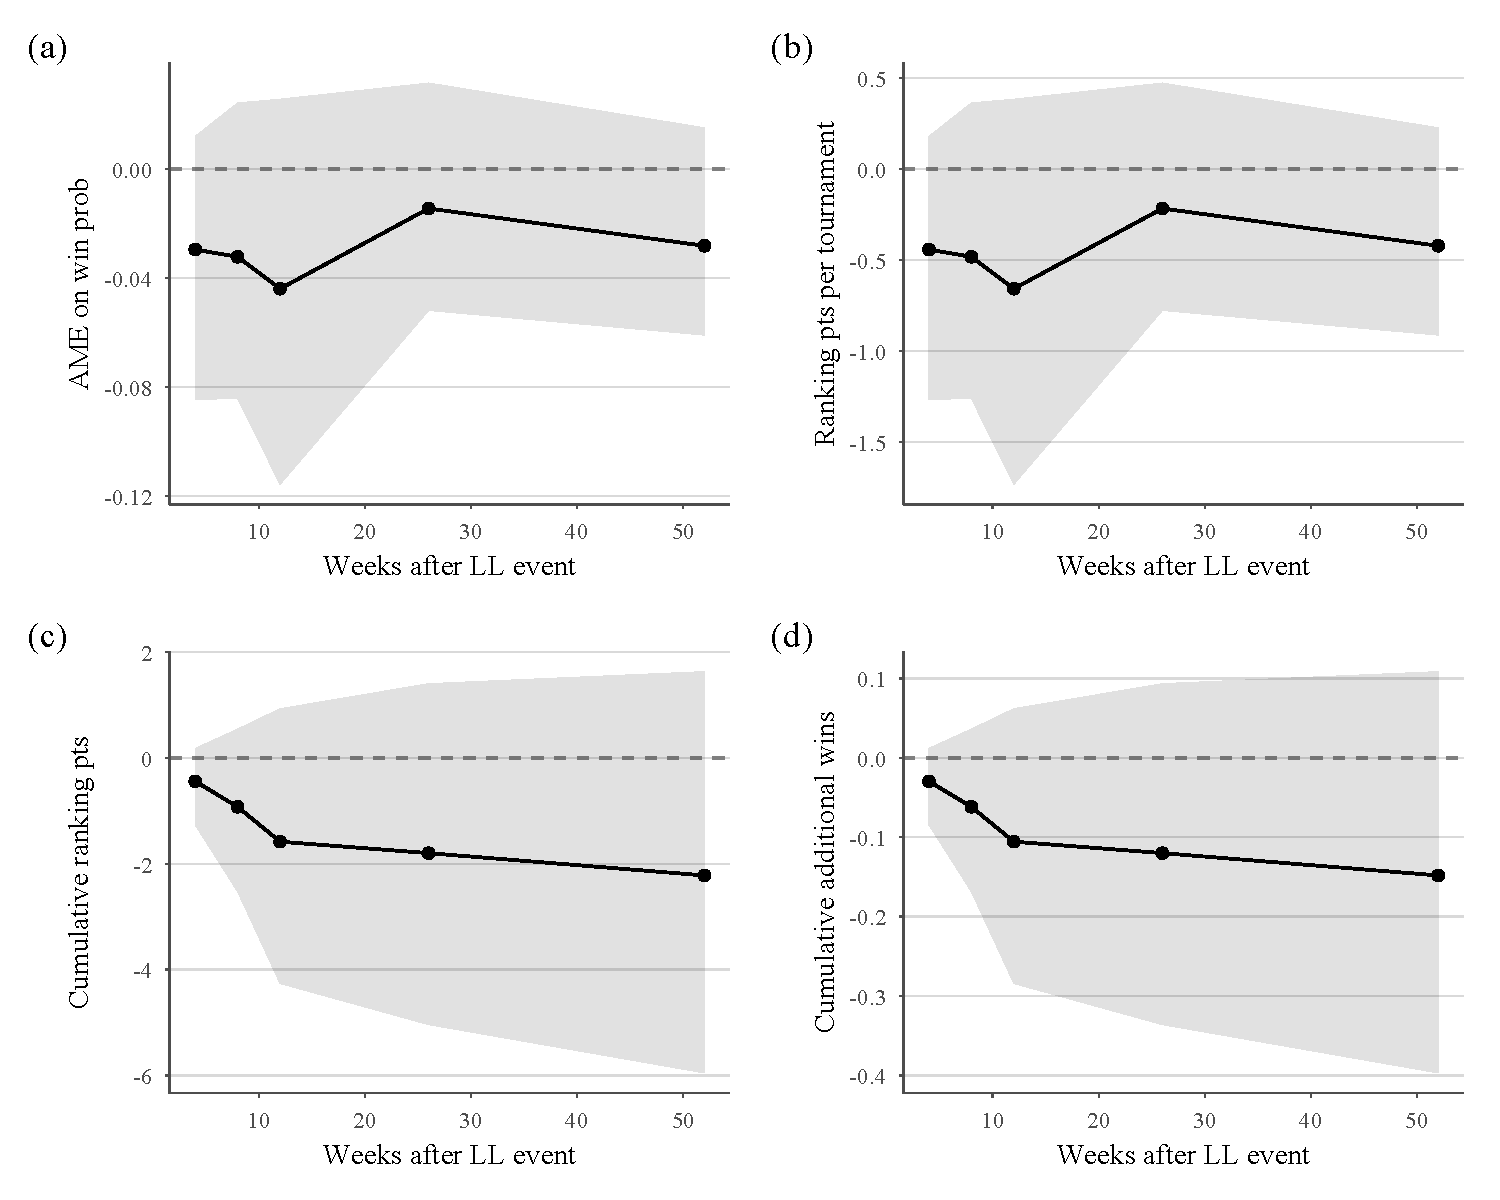
\includegraphics[width=0.95\textwidth]{../Figures/fig_delta_horizon_gs_atp.pdf}
\caption{Match-Level Treatment Effects by Calendar Horizon: Grand Slam ATP}
\label{fig:delta_horizon_gs_atp}
\begin{minipage}{0.9\textwidth}
\vspace{0.5em}
\footnotesize \textit{Notes.} Four panels report the match-level LL treatment effect and derived tournament-level quantities at calendar horizons of 4, 8, 12, 26, and 52 weeks after the LL-granting event. Panel (a): average marginal effect on match win probability. Panel (b): expected additional ranking points per tournament. Panel (c): cumulative expected ranking points through each horizon. Panel (d): cumulative expected additional wins through each horizon. Grand Slam ATP sample ($N = 8{,}543$ matches, 130 players). Shaded bands are 95\% confidence intervals from player-level block bootstrap (200 replications).
\end{minipage}
\end{figure}

\begin{figure}[htbp]
\centering
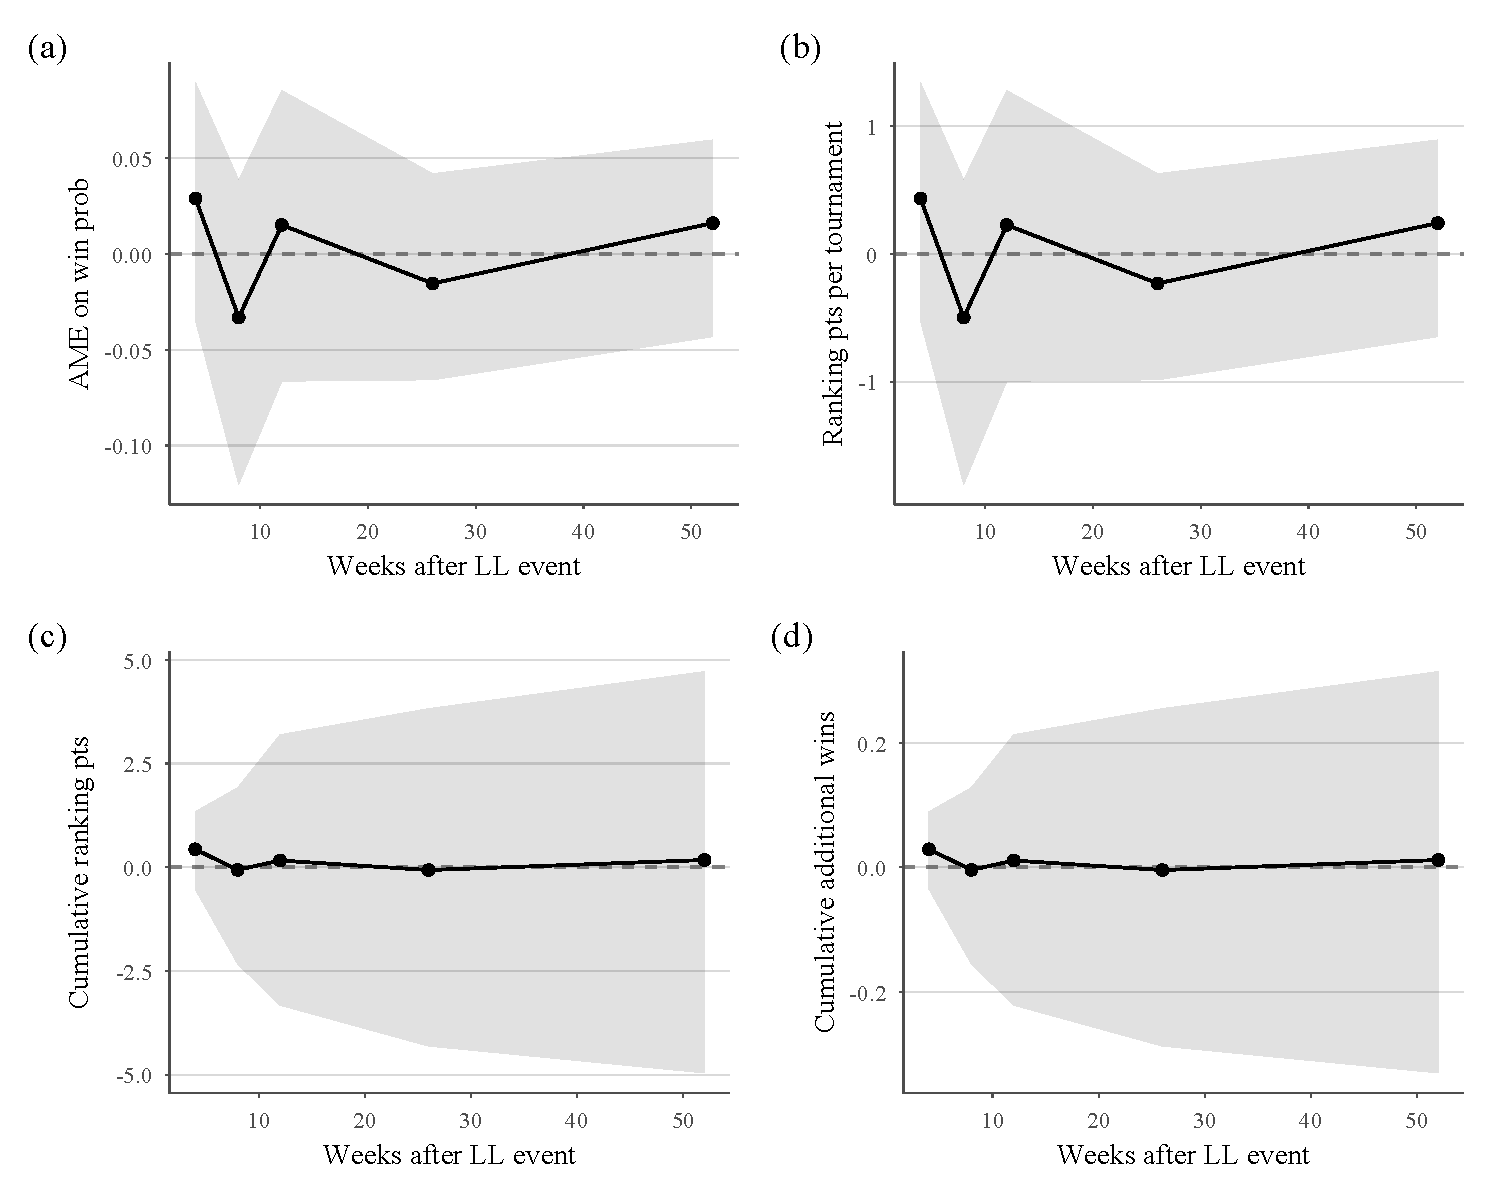
\includegraphics[width=0.95\textwidth]{../Figures/fig_delta_horizon_gs_wta.pdf}
\caption{Match-Level Treatment Effects by Calendar Horizon: Grand Slam WTA}
\label{fig:delta_horizon_gs_wta}
\begin{minipage}{0.9\textwidth}
\vspace{0.5em}
\footnotesize \textit{Notes.} Same specification as Figure~\ref{fig:delta_horizon_gs_atp}. Grand Slam WTA sample ($N = 5{,}391$ matches, 98 players). Shaded bands are 95\% confidence intervals from player-level block bootstrap (200 replications).
\end{minipage}
\end{figure}

\begin{figure}[htbp]
\centering
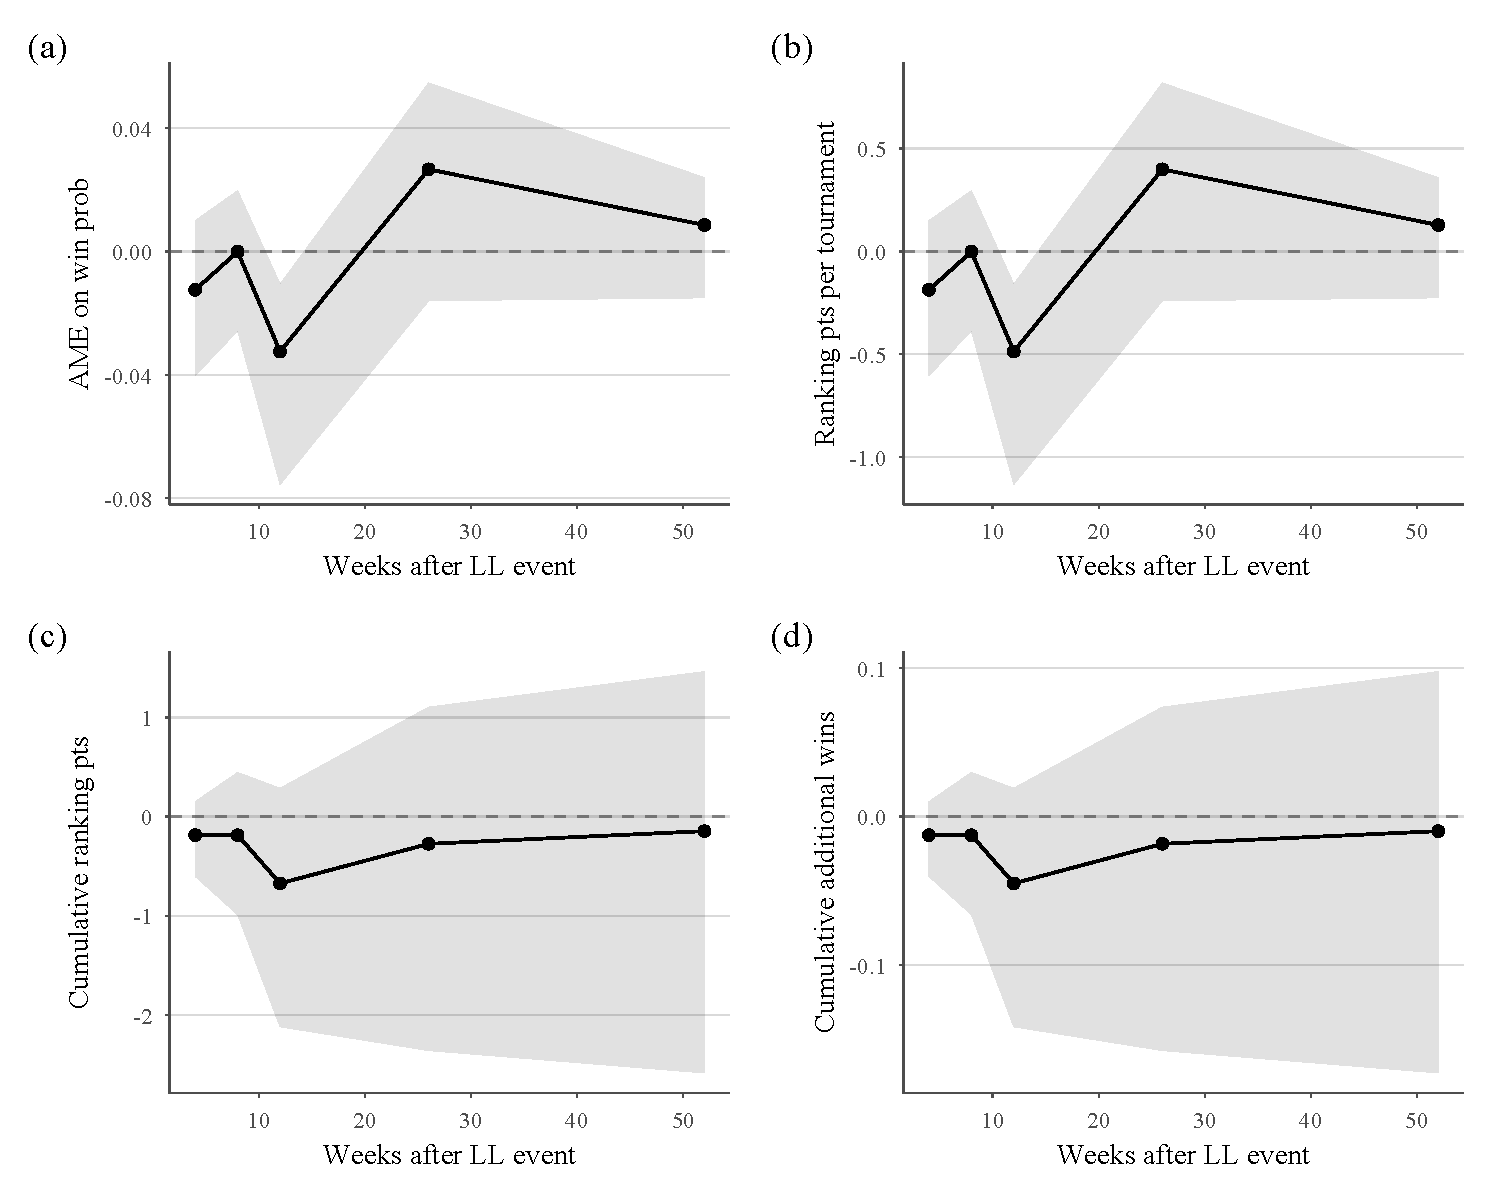
\includegraphics[width=0.95\textwidth]{../Figures/fig_delta_horizon_nongs_atp.pdf}
\caption{Match-Level Treatment Effects by Calendar Horizon: Non-Grand-Slam ATP}
\label{fig:delta_horizon_nongs_atp}
\begin{minipage}{0.9\textwidth}
\vspace{0.5em}
\footnotesize \textit{Notes.} Same specification as Figure~\ref{fig:delta_horizon_gs_atp}, with control function correction for endogenous LL assignment. Non-Grand-Slam ATP sample ($N = 113{,}189$ matches, 838 players). Shaded bands are 95\% confidence intervals from player-level block bootstrap (200 replications).
\end{minipage}
\end{figure}

\begin{figure}[htbp]
\centering
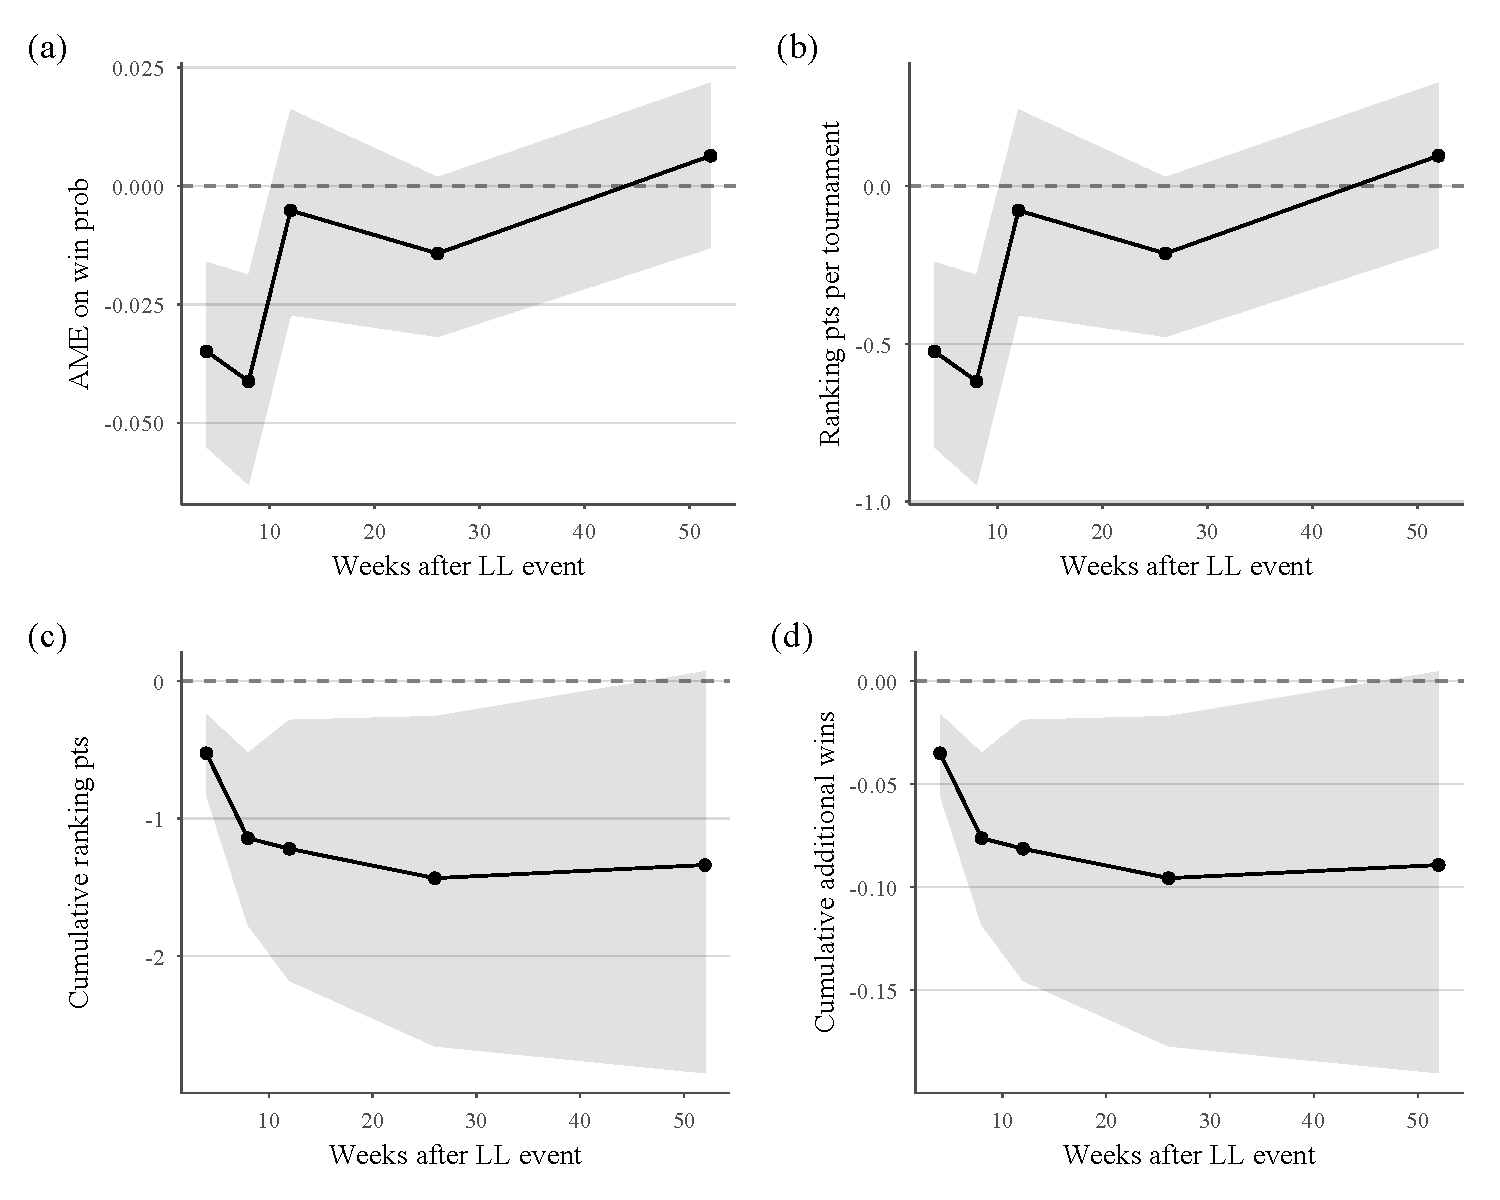
\includegraphics[width=0.95\textwidth]{../Figures/fig_delta_horizon_nongs_wta.pdf}
\caption{Match-Level Treatment Effects by Calendar Horizon: Non-Grand-Slam WTA}
\label{fig:delta_horizon_nongs_wta}
\begin{minipage}{0.9\textwidth}
\vspace{0.5em}
\footnotesize \textit{Notes.} Same specification as Figure~\ref{fig:delta_horizon_nongs_atp}. Non-Grand-Slam WTA sample ($N = 80{,}168$ matches, 747 players). Shaded bands are 95\% confidence intervals from player-level block bootstrap (200 replications).
\end{minipage}
\end{figure}

\begin{figure}[htbp]
\centering
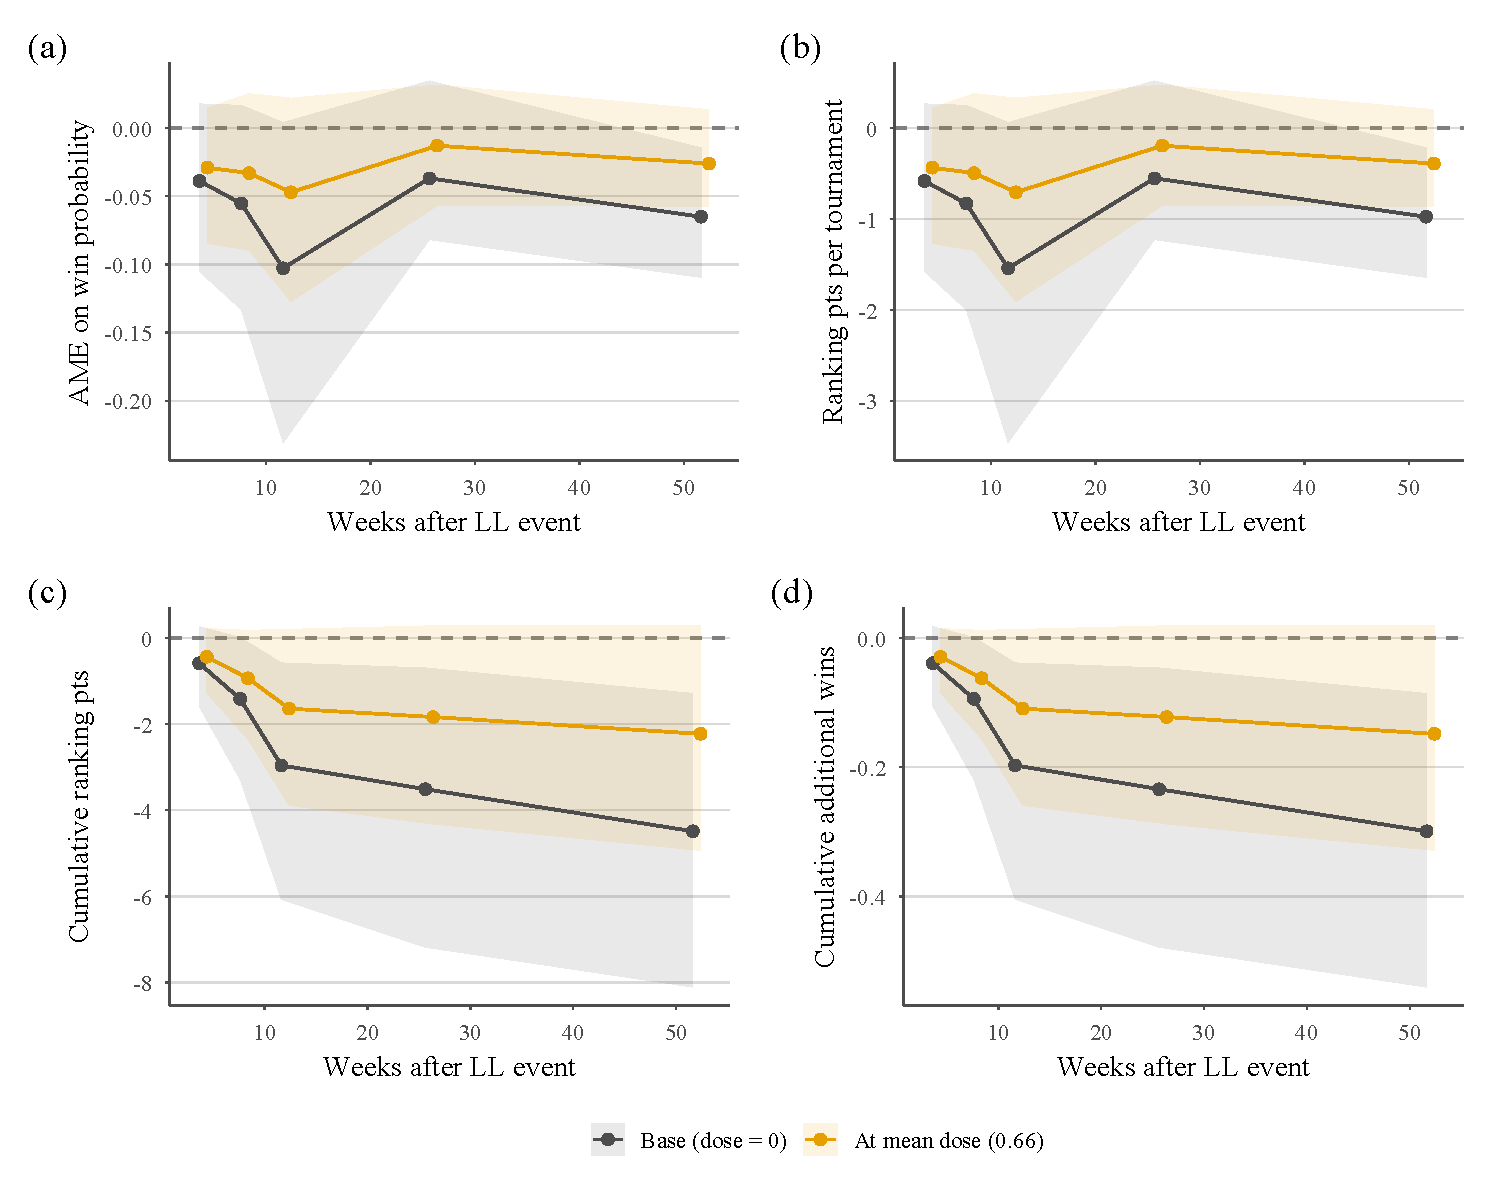
\includegraphics[width=0.95\textwidth]{../Figures/fig_delta_horizon_dose_gs_atp.pdf}
\caption{Match-Level Treatment Effects by Horizon and Performance Dose: Grand Slam ATP}
\label{fig:delta_horizon_dose_gs_atp}
\begin{minipage}{0.9\textwidth}
\vspace{0.5em}
\footnotesize \textit{Notes.} Same four-panel format as Figure~\ref{fig:delta_horizon_gs_atp}. Two series: base effect (dose $= 0$, solid) and effect at mean dose among treated (dashed). Grand Slam ATP sample. Shaded bands are 95\% bootstrap CIs.
\end{minipage}
\end{figure}

\begin{figure}[htbp]
\centering
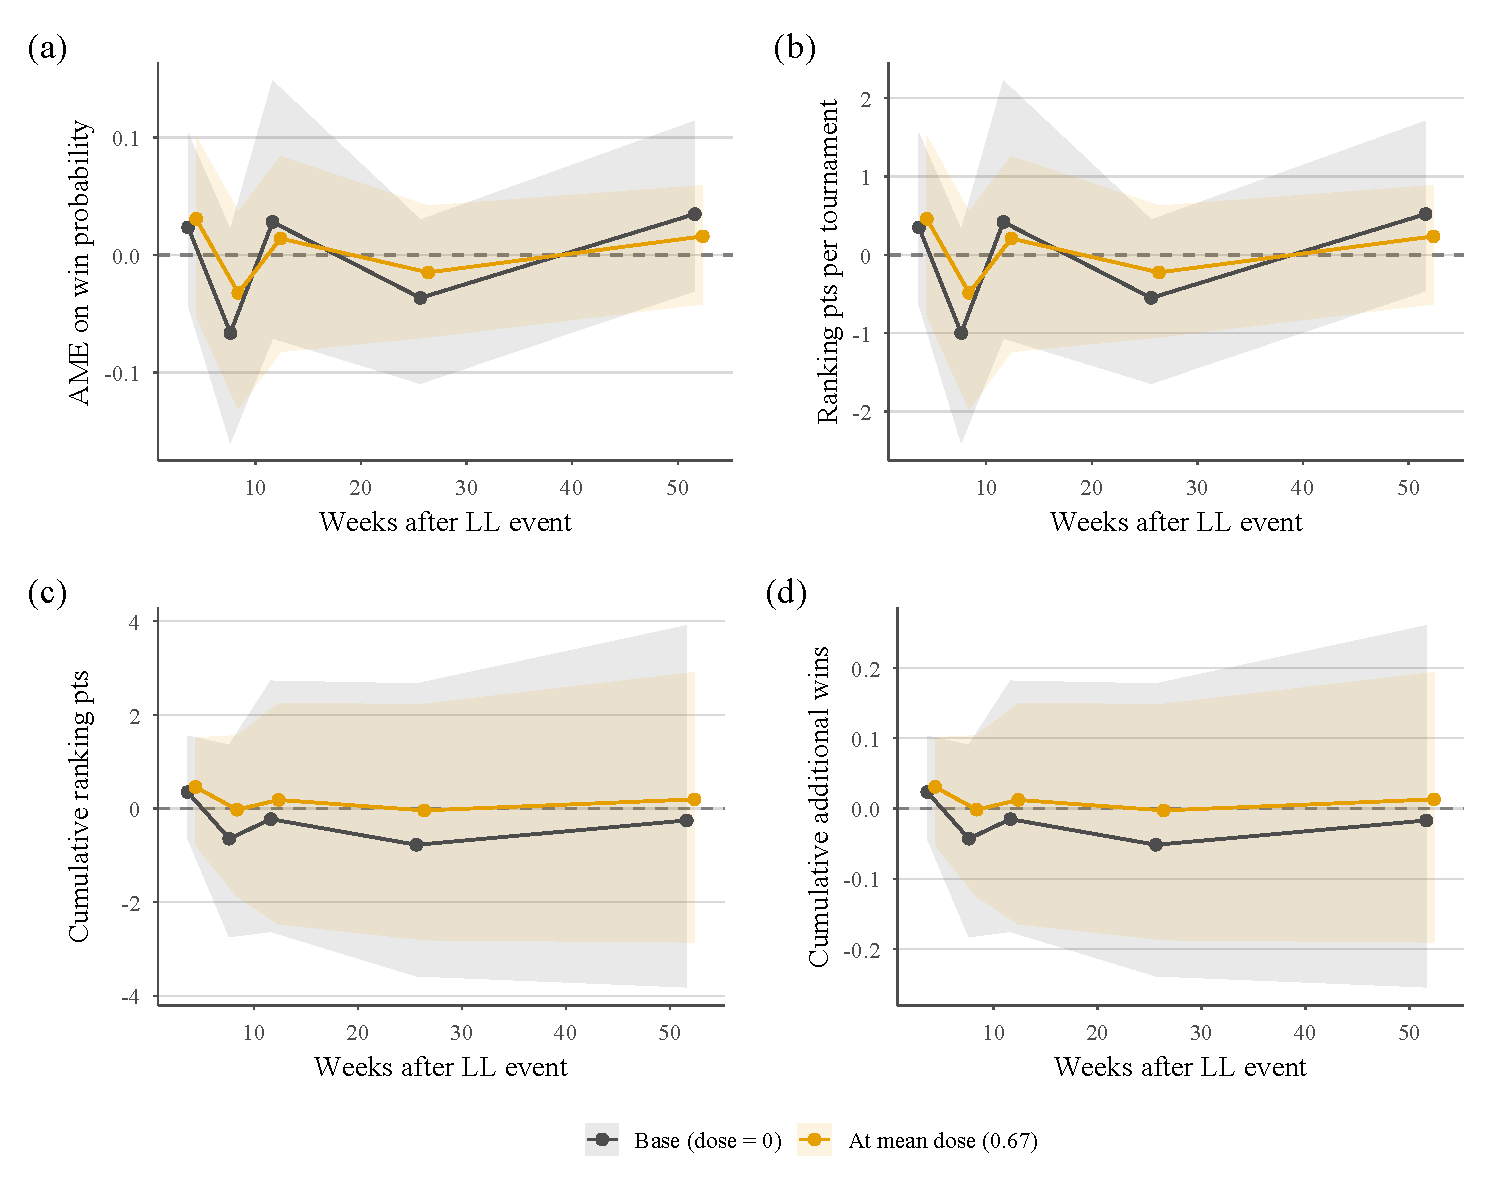
\includegraphics[width=0.95\textwidth]{../Figures/fig_delta_horizon_dose_gs_wta.pdf}
\caption{Match-Level Treatment Effects by Horizon and Performance Dose: Grand Slam WTA}
\label{fig:delta_horizon_dose_gs_wta}
\begin{minipage}{0.9\textwidth}
\vspace{0.5em}
\footnotesize \textit{Notes.} Same specification as Figure~\ref{fig:delta_horizon_dose_gs_atp}. Grand Slam WTA sample. Shaded bands are 95\% bootstrap CIs.
\end{minipage}
\end{figure}

\begin{figure}[htbp]
\centering
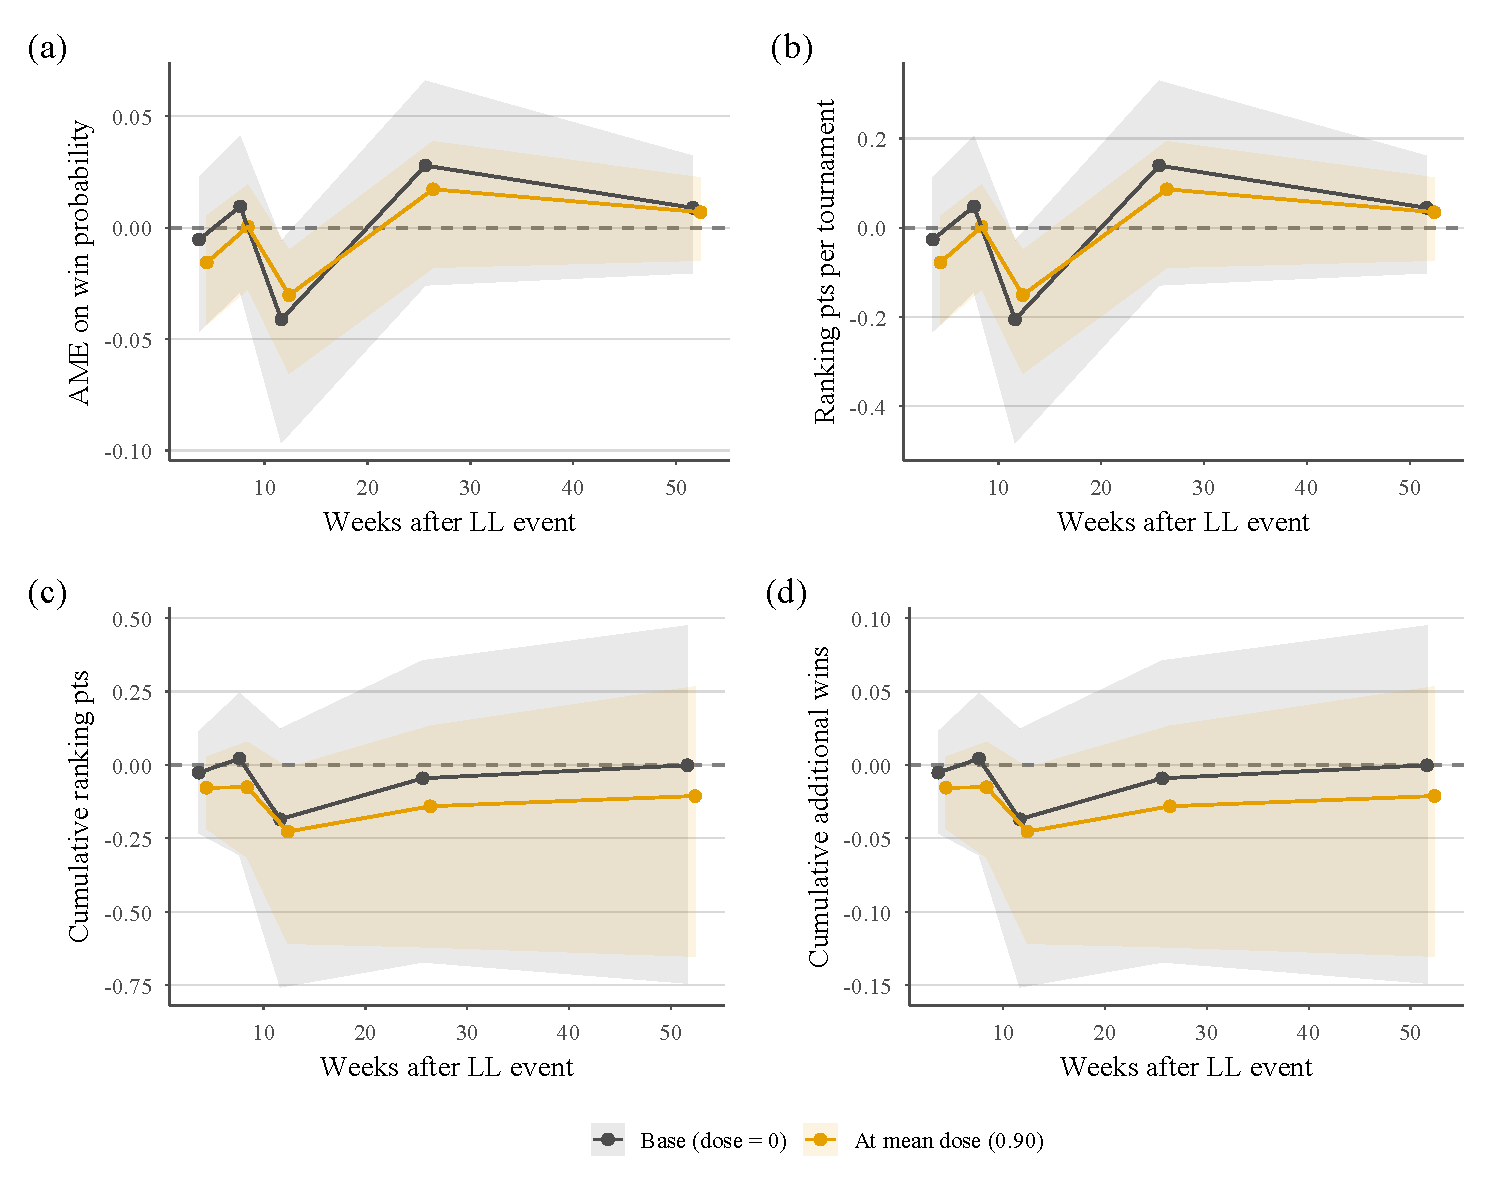
\includegraphics[width=0.95\textwidth]{../Figures/fig_delta_horizon_dose_nongs_atp.pdf}
\caption{Match-Level Treatment Effects by Horizon and Performance Dose: Non-Grand-Slam ATP}
\label{fig:delta_horizon_dose_nongs_atp}
\begin{minipage}{0.9\textwidth}
\vspace{0.5em}
\footnotesize \textit{Notes.} Same specification as Figure~\ref{fig:delta_horizon_dose_gs_atp}, with control function correction for endogenous LL assignment. Non-Grand-Slam ATP sample. Shaded bands are 95\% bootstrap CIs.
\end{minipage}
\end{figure}

\begin{figure}[htbp]
\centering
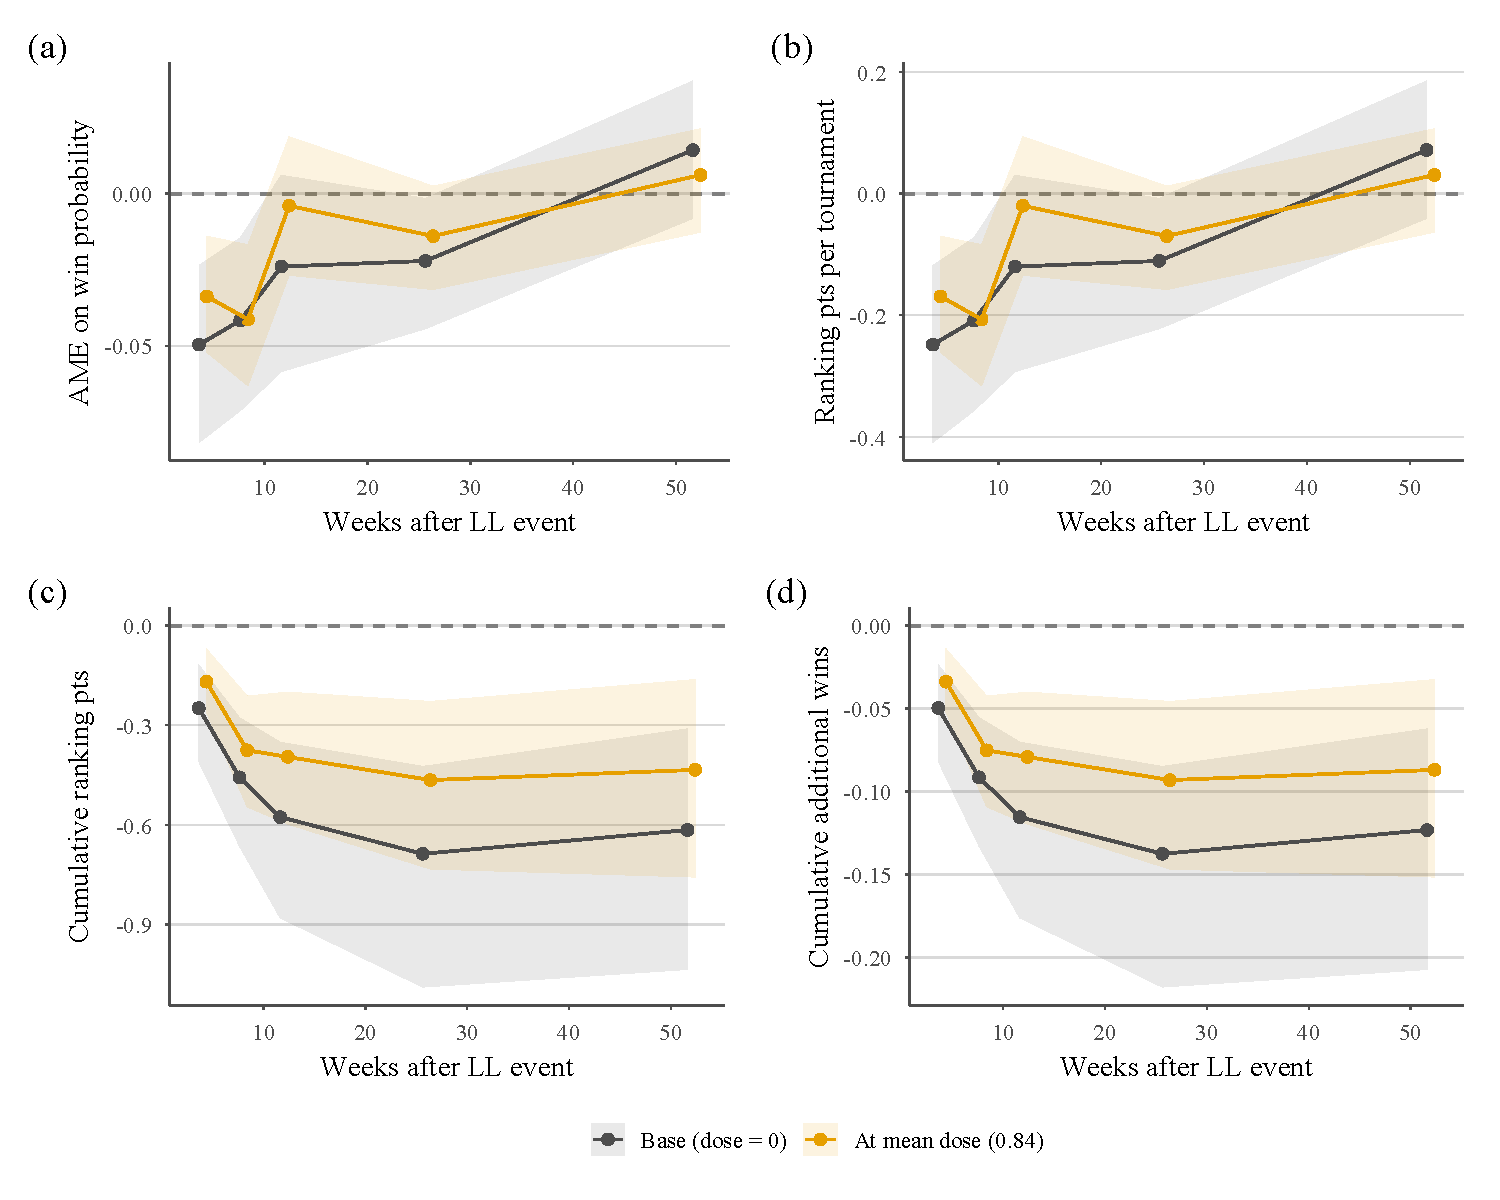
\includegraphics[width=0.95\textwidth]{../Figures/fig_delta_horizon_dose_nongs_wta.pdf}
\caption{Match-Level Treatment Effects by Horizon and Performance Dose: Non-Grand-Slam WTA}
\label{fig:delta_horizon_dose_nongs_wta}
\begin{minipage}{0.9\textwidth}
\vspace{0.5em}
\footnotesize \textit{Notes.} Same specification as Figure~\ref{fig:delta_horizon_dose_nongs_atp}. Non-Grand-Slam WTA sample. Shaded bands are 95\% bootstrap CIs.
\end{minipage}
\end{figure}

\paragraph{Link to reduced-form results.} The GS-ATP estimate ($\hat{\delta} = -0.123$, $p = 0.119$) is consistent with the reduced-form findings in Section~\ref{sec:results}: positive access effects and null Elo effects. LL entry provides additional tournament appearances through the ranking system, but treated players perform neither better nor worse than controls once opponent strength and context are held constant. The ranking point gains documented in Section~\ref{sec:results} come purely from additional tournament participation---more draws entered, more matches played---not from playing better or worse once in the draw. The GS-WTA estimate ($\hat{\delta} = +0.034$, $p = 0.760$) is also a null, reinforcing the access-not-ability interpretation. The WTA dynamic results in Section~\ref{sec:results} show marginally significant Elo gains at short horizons; the absence of a corresponding match-level effect suggests that those Elo gains may reflect favorable opponent draws in additional tournaments rather than improved competitive skill per se.

At non-Grand-Slam events, the control-function estimates yield $\hat{\delta} = +0.033$ on the ATP tour (bootstrap SE $= 0.050$, $p = 0.513$; 113,189 matches from 838 players) and $\hat{\delta} = -0.060$ on the WTA tour (bootstrap SE $= 0.032$, $p = 0.061$; 80,168 matches from 747 players). The ATP non-GS estimate is small and insignificant, consistent with the Grand Slam null. The WTA non-GS estimate is marginally significant and negative, an unexpected result that may reflect selection: WTA LL recipients at non-GS events who receive their slot by ranking (rather than lottery) may face systematically tougher early-round opponents, producing a mechanical disadvantage in subsequent match outcomes. This estimate should be interpreted with caution and does not alter the overall conclusion that match-level performance effects are generally null across tours and identification strategies. These results are reported in Appendix~\ref{app:nongs_tournament}.

\subsection{Reconciling with the Existing Literature}
\label{sec:mechanisms_reconciling}

\citet{Maity2025_early_career_sports} report positive correlations between lucky loser entry and career outcomes. The Grand Slam tournament performance model, which exploits the lottery for identification, finds no detectable effect of LL entry on match-level win probability on either tour: $\hat{\delta} = -0.123$ ($p = 0.119$) on the ATP tour and $\hat{\delta} = +0.034$ ($p = 0.760$) on the WTA tour. The null on both tours is consistent with the access-not-ability interpretation: the correlational finding in \citet{Maity2025_early_career_sports} likely reflects the additional tournament participation that LL entry generates, not improved competitive performance per se. The causal estimates here establish that LL entry does not detectably change match-level win probability conditional on opponent strength.

The initial conditions literature finds persistent effects of early-career shocks \citep{Oyer2006_initial_placement, Oreopoulos2012_graduating_recession}. The present results are consistent with these findings on the access dimension: LL entry causes persistent changes in the number and type of tournaments a player enters. The ability dimension is null on both tours: Elo is flat, and match-level performance conditional on opponent strength is unchanged. This contrast suggests that persistence depends on market transparency: in professional tennis, where performance is measured match by match and rankings update weekly, ability reasserts itself within a year. The access channel alone is sufficient to generate the ranking point gains and tournament entry effects documented in Section~\ref{sec:results}.
